\chapter{Dane}
\section{Charakterystyka}
Dane pozyskane do eksperymentów pochodziły z ogólnodostępnych portali takich jak YouTube. Wybór sekwencji wideo dokonano tak, aby realizowany algorytm jak najlepiej spełniał swoje funkcje. W tym celu starano się spełnić następujące ograniczenia:
\begin{itemize}
\item Ujęcia pochodzące kamery, której pozycja nie zmienia się w dużym stopniu w czasie. Aczkolwiek możliwe są jej obroty o dowolny kąt.
\item Ujęcia z dużą ilością elementów poruszających się tj. samochody, piesi, statki itp.
\item Ujęcia ruchome o możliwie niskiej dystorsji soczewki (zaproponowane rozwiązanie całkowicie pomija to zagadnienie)
\end{itemize}
\section{Przykłady} \label{samples}

\begin{figure}[H]
	\centering
		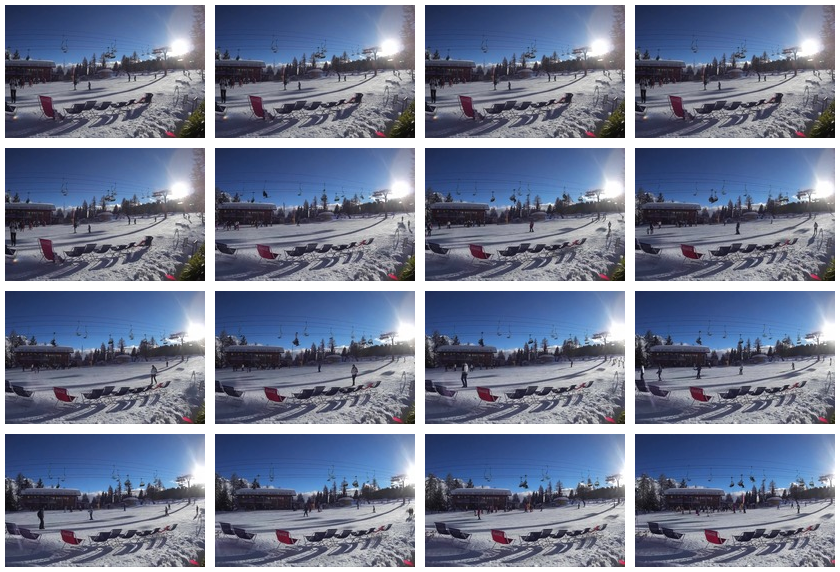
\includegraphics[width=0.75\linewidth]{img/ski_cuted_frames_tile.png}
	\caption[Sekwencja zdjęć 'ski'.]{Przykładowa sekwencja zdjęć 'ski'.}
	\label{fig:binary}
\end{figure}

\begin{figure}[H]
	\centering
		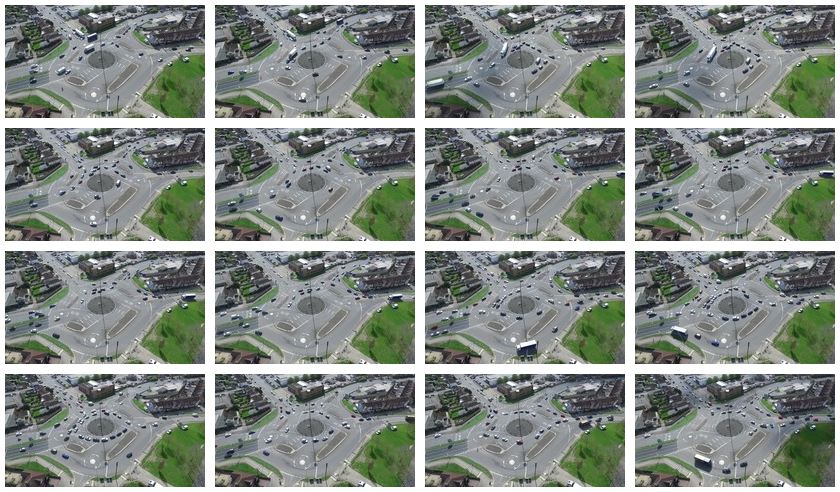
\includegraphics[width=0.75\linewidth]{img/roundabout_frames_tile.png}
	\caption[Sekwencja zdjęć 'roundabout'.]{Przykładowa sekwencja zdjęć 'roundabout'.}
	\label{fig:binary}
\end{figure}

\begin{figure}[H]
	\centering
		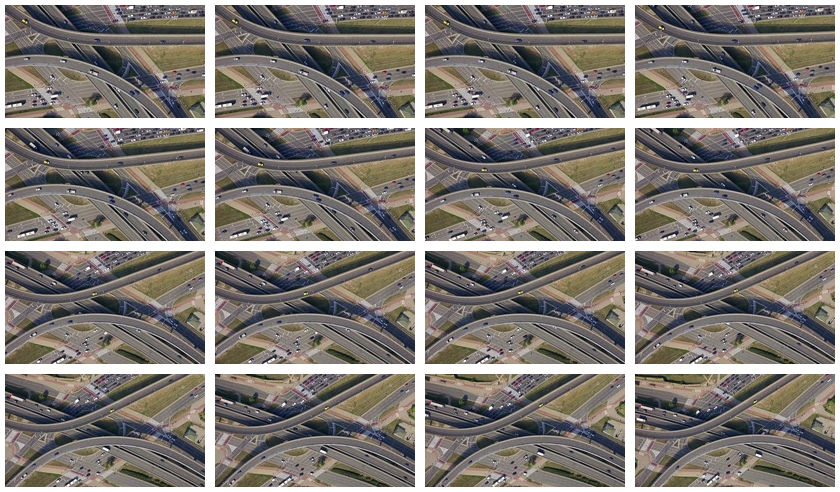
\includegraphics[width=0.75\linewidth]{img/warsaw_cuted_frames_tile.png}
	\caption[Sekwencja zdjęć 'warsaw'.]{Przykładowa sekwencja zdjęć 'warsaw'.}
	\label{fig:binary}
\end{figure}

\begin{figure}[H]
	\centering
		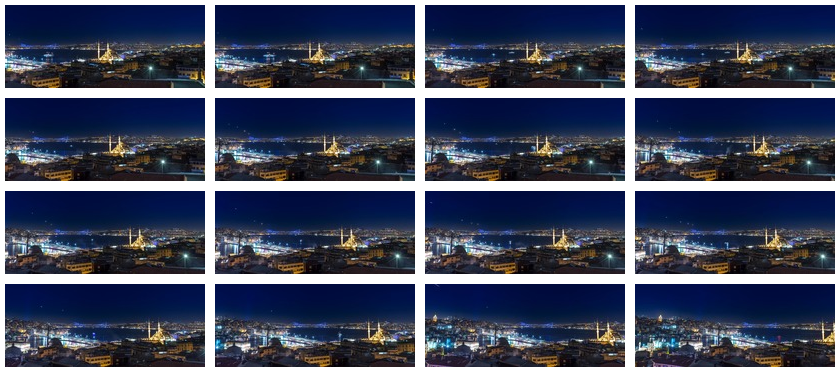
\includegraphics[width=0.75\linewidth]{img/istanbul_cuted_frames_tile.png}
	\caption[Sekwencja zdjęć 'istanbul'.]{Przykładowa sekwencja zdjęć 'istanbul'.}
	\label{fig:binary}
\end{figure}